\section{Performance Evaluation}
\label{sec:evaluation}
In this section, we evaluate the performance of the proposed low-complexity dispatching policy $\tilde{\Policy}$ by numerical simulations.
The experiment setup and performance benchmarks are elaborated in Section \ref{subsec:setup}.
The simulation results are illustrated in Section \ref{subsec:basic}.
The sensitivity study on parameters is also applied to provide some insights on the robustness of the proposed policy in Section \ref{subsec:advance}.

\subsection{Experiment Setup}
\label{subsec:setup}
In the simulation, there are $K=5$ APs, $M=3$ edge servers and $J=5$ type of jobs in the system.
The edge servers are all fully-accessible to all the APs, i.e., $\esSet_{k}=\esSet$ ($\forall k\in\apSet$).

The time slot duration is 50 milliseconds and one broadcast interval consists of $t_{B}=20$ time slots, i.e., its duration is $1$ second.
% The distributions of arrival rate, uploading time and processing time are generated randomly.
The maximum uploading time is $3$ seconds, i.e., $\Xi = 3t_B$, and the distribution of $\mathbb{U}_{k,m,j}(\Xi)$ is arbitrarily generated within the support $[0, \Xi]$.
The expected computation time $c_{m,j}$ is also randomly generated in the range $[30,50]$ with the unit of time slot.

Each queue for VMs on edge server is with maximum queue length $L_{max}=20$, i.e., there would be at most $100$ jobs on one edge server.
The arrival rate is arbitrarily generated around $0.03$ for each AP.
The discount factor $\gamma$ is $0.95$ and the penalty weight $\beta$ is $20$.
% The arrival rate is taken as small probability with enough APs in the system, and correspondingly enough edge servers for the processing.

%-----------------------------------------------------------------------------------------------%
\begin{figure}[ht!]                                                                             %
    \centering                                                                                  %
    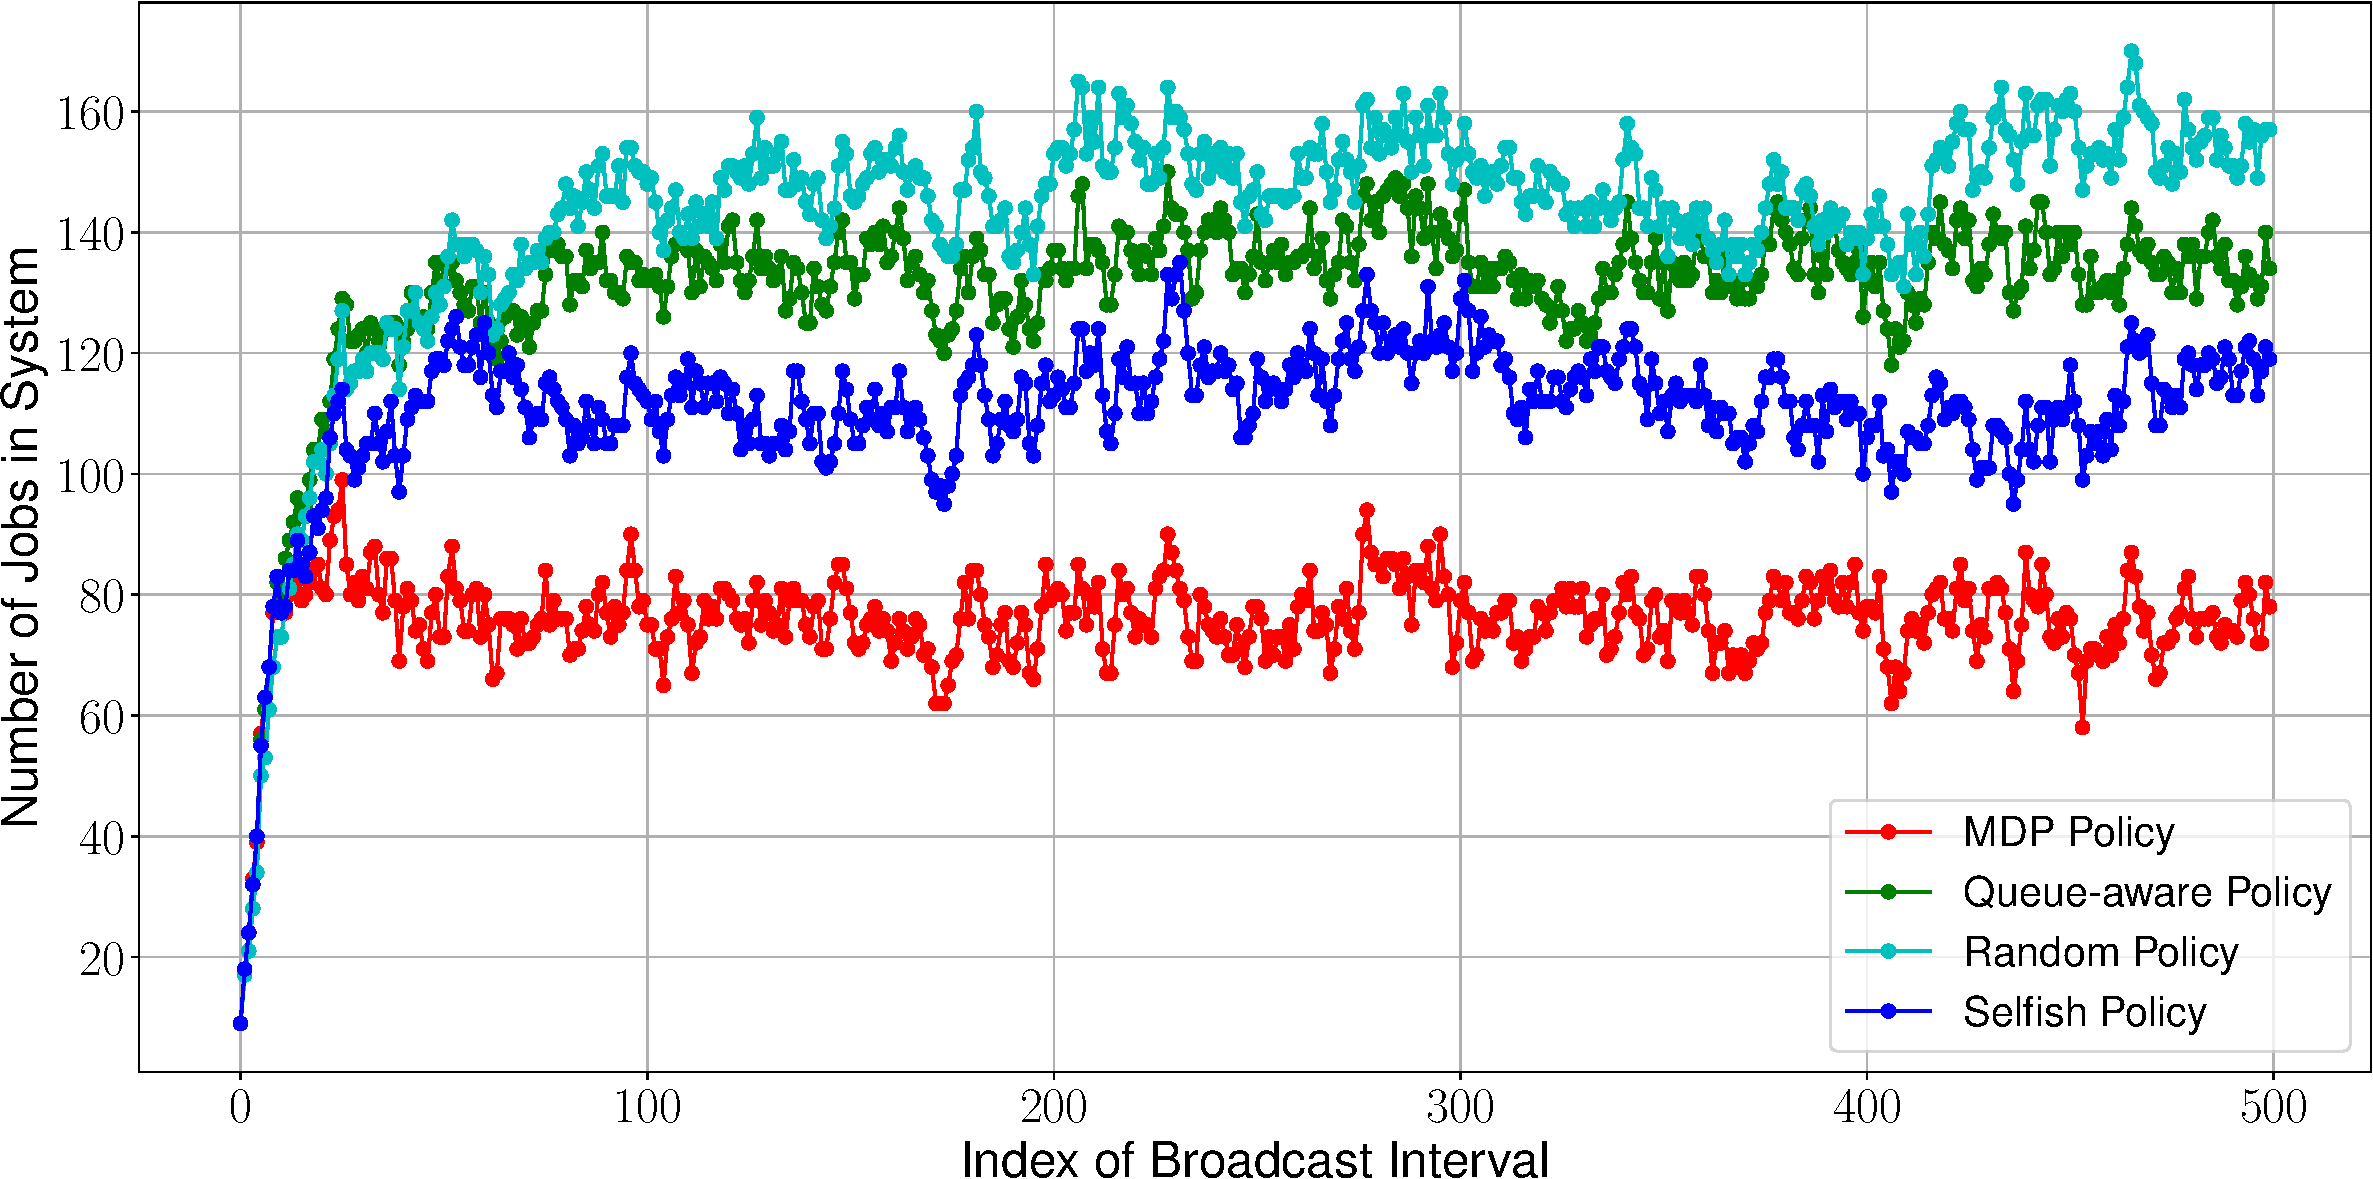
\includegraphics[width=0.45\textwidth]{41122-timeline-number-alter.pdf}                     %
    \caption{Illustration of number of jobs on all the APs and edge servers over time.}
    \label{fig:general_timeline}                                                                %
\end{figure}                                                                                    %
%-----------------------------------------------------------------------------------------------%

%NOTE: Benchmark Elaboration
We compare the proposed algorithm with other three benchmarks which are listed as follows. For each type of jobs,
\begin{itemize}
    \item \textbf{Random Dispatching Policy}:
            Randomly choose a dispatching edge server in a time slot; 
    \item \textbf{Selfish Policy}:
            Always choose the edge server with the minimum expected uploading time together with the expected processing time;
    \item \textbf{Queue-aware Policy}:
            Always choose the edge server with the minimum expected uploading time together with the expected processing time and queueing time based on the observation of outdated queue states.
\end{itemize}
Specifically, we choose the \emph{Selfish Policy} which is state-invariant as the initial policy for our proposed algorithm.
The explicit definition is given as follows.
\begin{policy}[Selfish Policy]
    \begin{align}
        \Baseline \define \Brace{ \Pi_{k} |\forall k\in\apSet }, \Pi_{k} \define \Brace{{\pi_{k,j}|\forall j\in\jSpace}}
    \end{align}
    where $\pi_{k,j} \define \arg\min_{m\in\esSet_{k}} u_{k,m,j} + c_{m,j}$.
\end{policy}

%NOTE: Basic Performance
\subsection{Performance Analysis}
\label{subsec:basic}
As illustrated in Fig.\ref{fig:bar_plot}, the simulation results straightly show that the proposed algorithm outperforms other benchmarks all the time with less pending jobs in the system, and the system converges fast from the start of the time.
The detailed analysis is provided in Fig.\ref{fig:bar_plot} where three metrics are taken to demonstrate different profiles of the benchmarks.
Firstly, the \emph{average cost} in Fig.\ref{fig:bar_plot}(a) shows that the proposed algorithm collects less cost than other algorithms within the same time duration.
% Moreover, 
Secondly, the \emph{average JCT} of all the jobs in Fig.\ref{fig:bar_plot}(b) resembles the shape of Fig.\ref{fig:bar_plot}(a) which proves the correctness of the cost function selection.
Finally, The \emph{average throughput} in Fig.\ref{fig:bar_plot}(c) is defined as the division of the total number of computed jobs (i.e., the jobs being accepted by edge servers and finishing the computation) over the time duration, and the results show that the proposed algorithm have the most of jobs computed in the system.

\delete{v20}{
    The CDF of cost is illustrated in Fig.\ref{fig:cdf_cost} where the cost of \emph{SQF policy} is nearly the same as the \emph{selfish policy}, however, the \emph{SQF policy} actually have very poor job departure rate (, throughput) compared with the other's.
    This is because the broadcast information is periodically and outdated, and SQF could not handle the penalty brought by job rejection properly.
    And we take \emph{CDF of number of jobs} other than \emph{CDF of cost} which could better reflect the performance of the average JCT target in the simulation when job rejection considered.
}

%-----------------------------------------------------------------------%
\begin{figure}[ht]                                                      %
    \centering                                                          %
    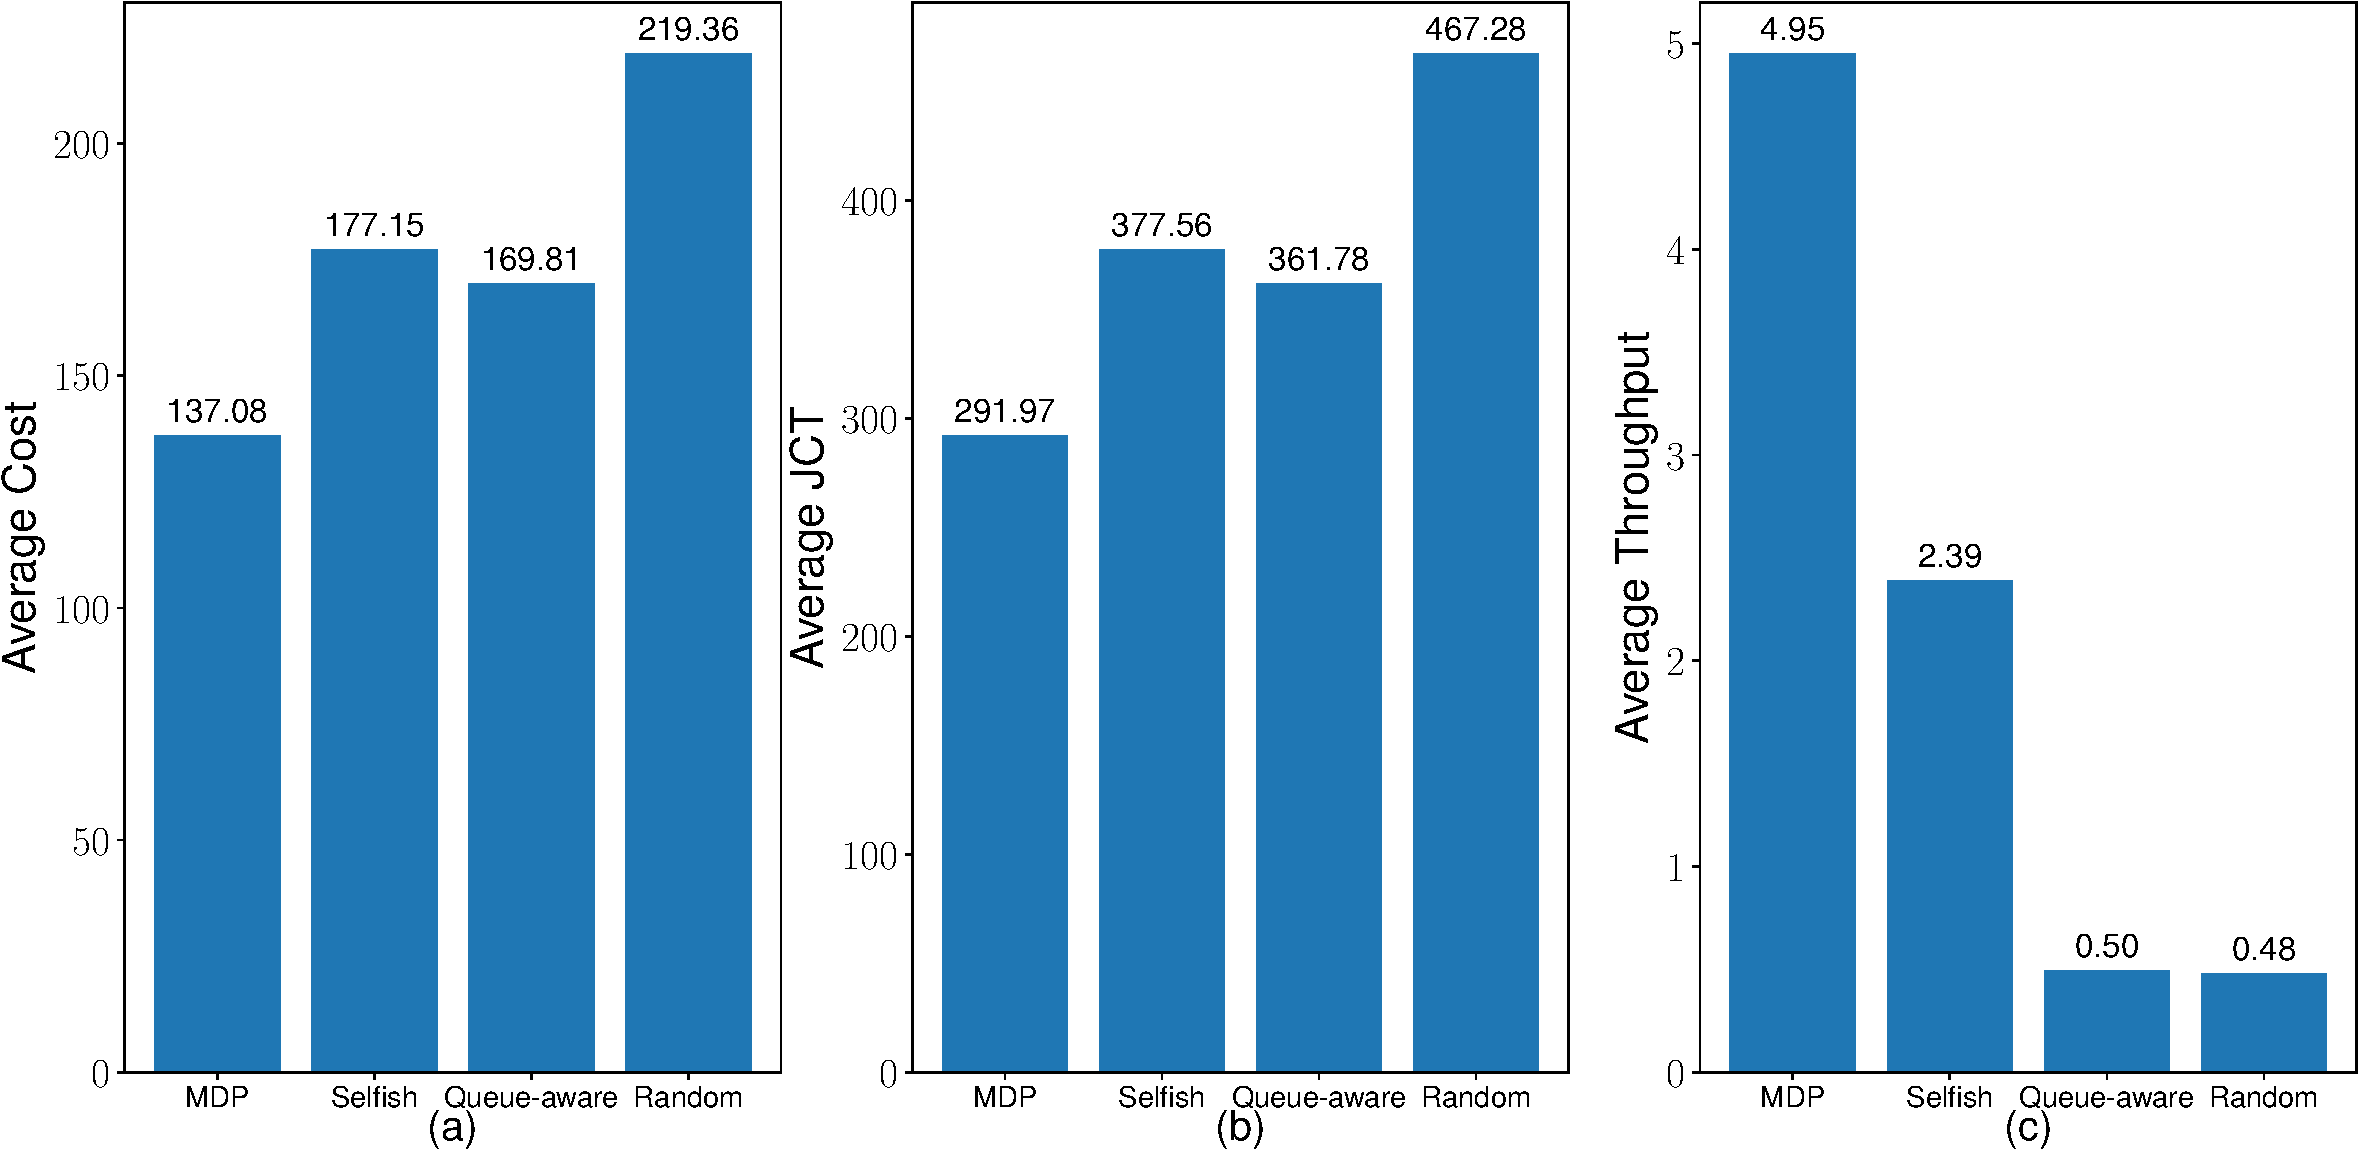
\includegraphics[width=0.45\textwidth]{41122-bar-graph-alter.pdf}         %
    \caption{Illustration of performance metrics comparison with benchmarks.}
    \label{fig:bar_plot}                                                %
\end{figure}                                                            %
%-----------------------------------------------------------------------%
% \begin{figure}[ht]                                                      %
%     \centering                                                          %
%     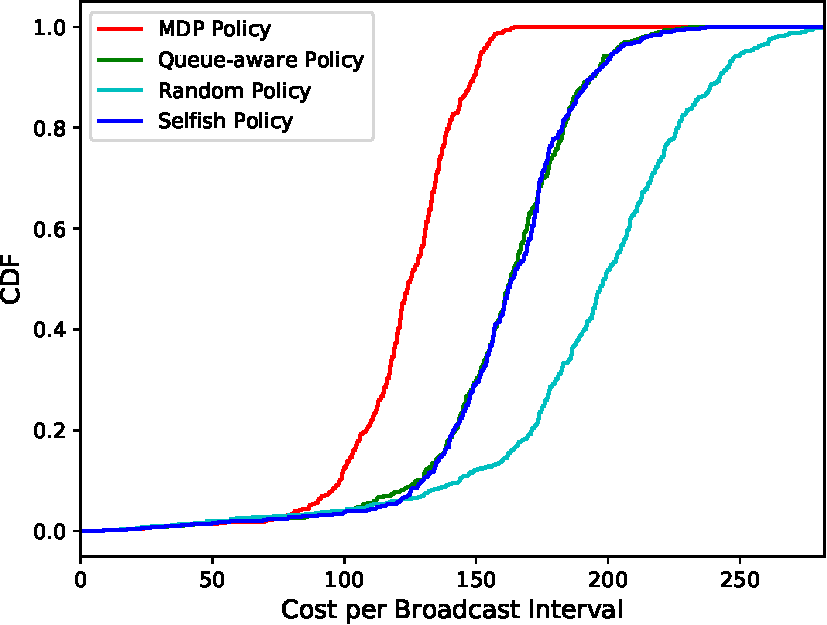
\includegraphics[width=0.45\textwidth]{41122-cdf-cost.pdf}          %
%     \caption{Illustration of performance metrics comparison with benchmarks.}
%     \label{fig:cdf_cost}                                                %
% \end{figure}                                                            %
%-----------------------------------------------------------------------%
%----------------------------------------------------------------------------------------%
\subsection{Sensitivity Study}
\label{subsec:advance}  

%FIXME: replace the graphs
%-----------------------------------------------------------------------------------%
\begin{figure*}[ht!]                                                                %
    \centering                                                                      %
    \begin{tabular}{ccc}                                                            %
        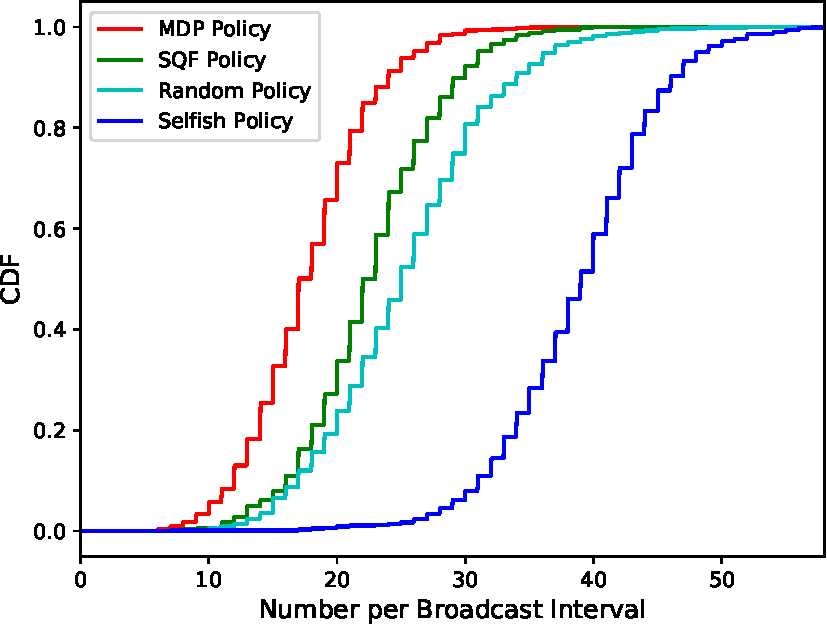
\includegraphics[width=0.30\textwidth]{LowPressure-d0.pdf}&                 %
        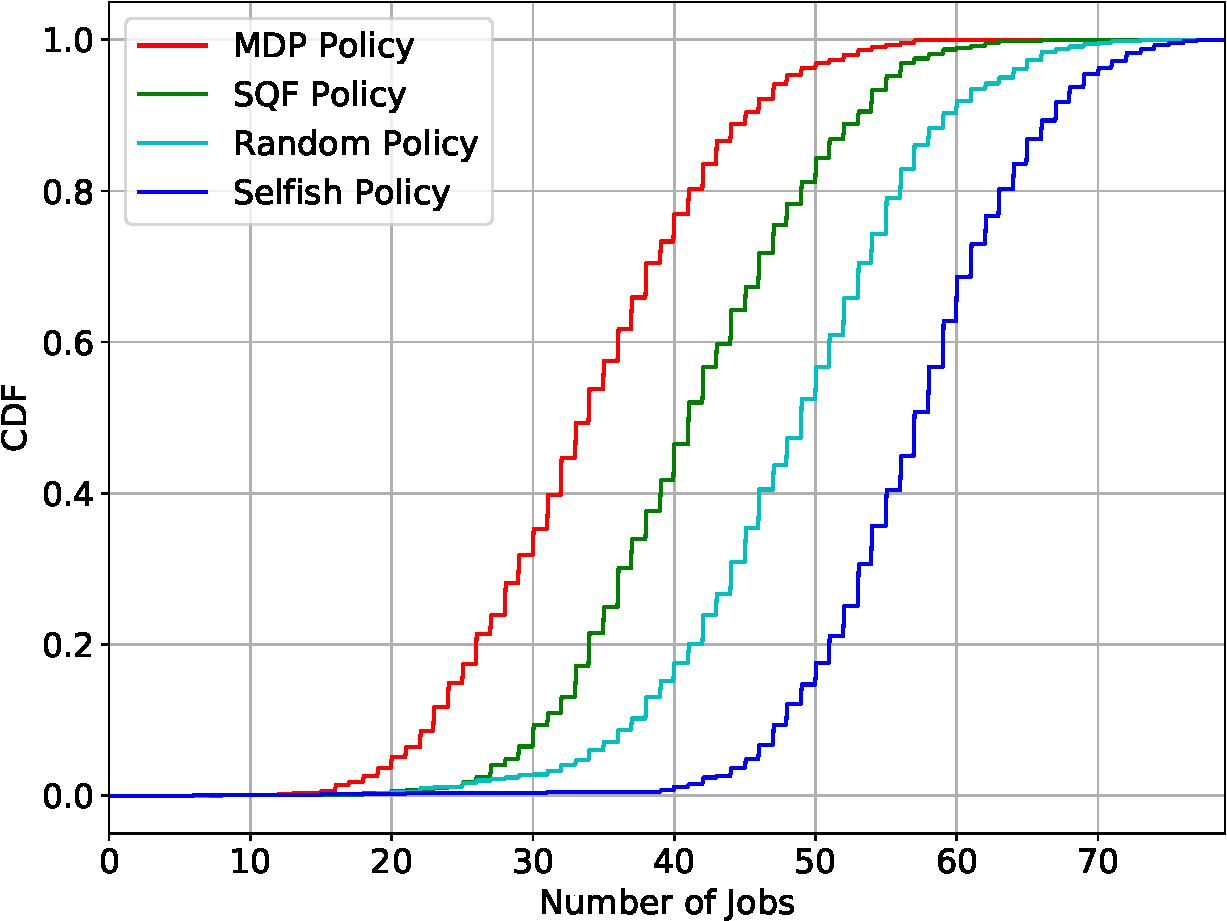
\includegraphics[width=0.30\textwidth]{LowPressure-d1.pdf}&                 %
        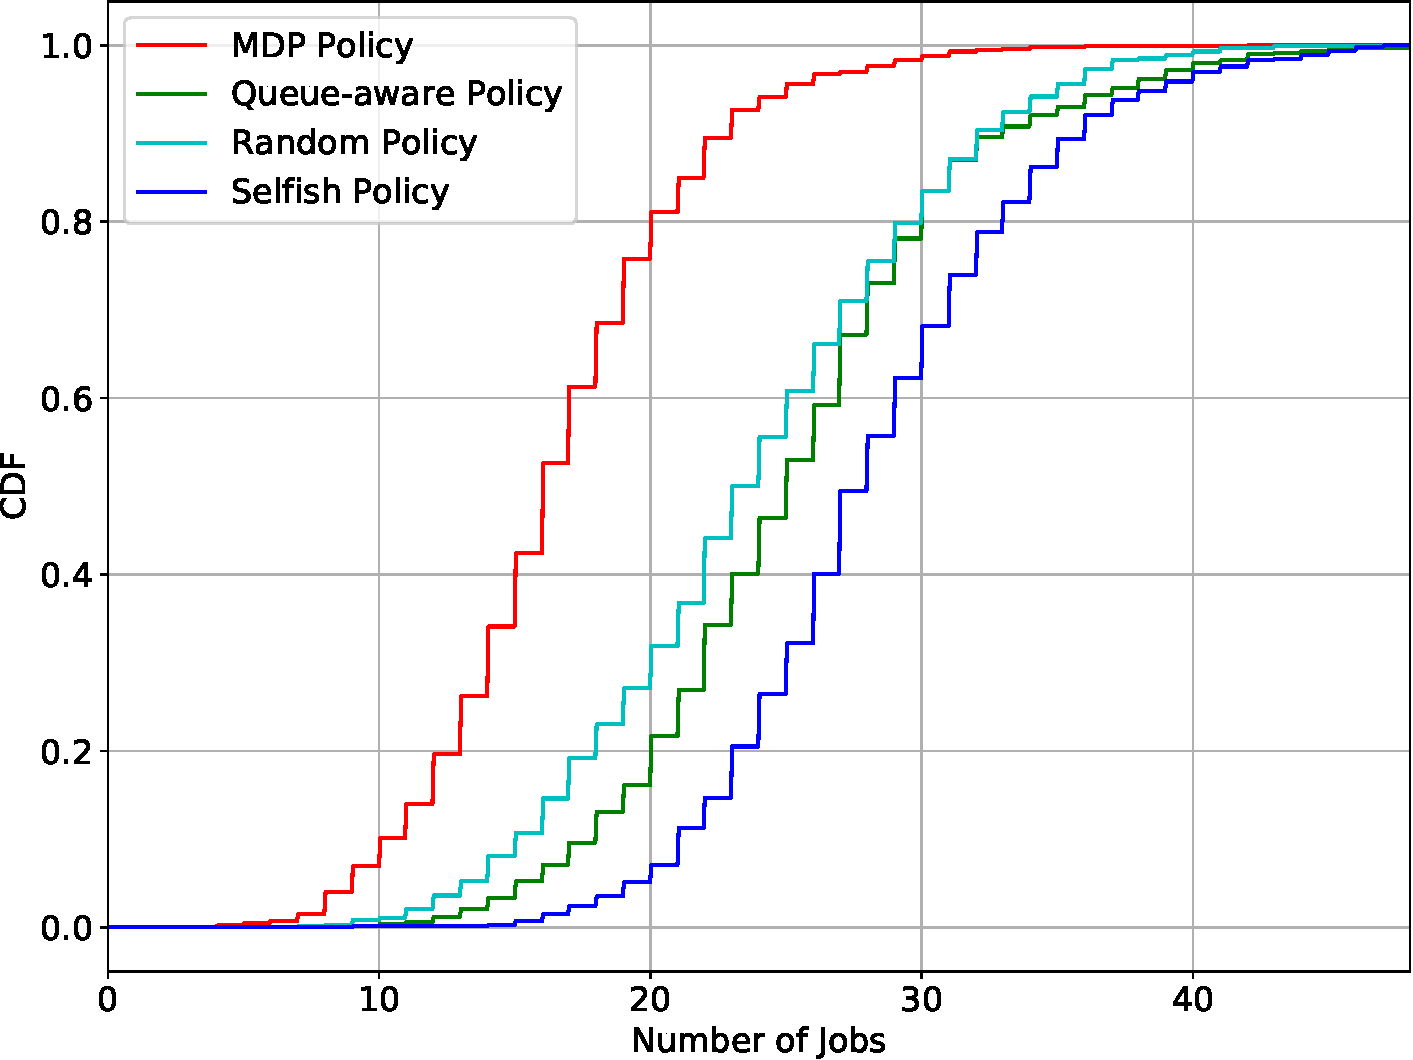
\includegraphics[width=0.30\textwidth]{LowPressure-d2.pdf}                  %
        \\                                                                          %
        {\small (a) No \brlatency} &                                                %
        {\small (b) Signaling latency in Section \ref{subsec:setup}} &
        {\small (c) Maximum \brlatency}                                             %
    \end{tabular}                                                                   %
    \caption{Evaluation of Information Staleness Impact on Algorithm Robustness.}
    \label{fig:ss_delay}                                                            %
\end{figure*}                                                                       %
%-----------------------------------------------------------------------------------%


%-------------------------------------------------------------------%
\begin{figure}[hbt]                                                 %
    \centering                                                      %
    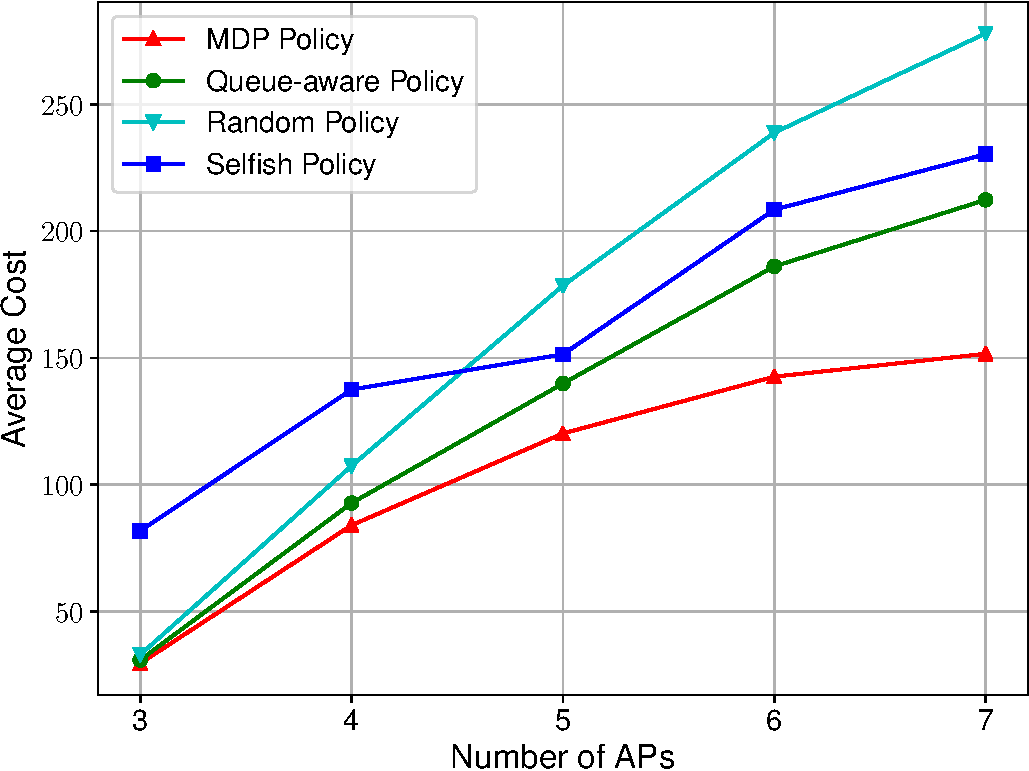
\includegraphics[width=0.45\textwidth]{Study-NumAPs.pdf}        %
    \caption{Illustration of impact of number of APs on algorithms.}
    \label{fig:ss_scale}                                            %
\end{figure}                                                        %
%-------------------------------------------------------------------%

%-------------------------------------------------------------------%
\begin{figure}[hbt]                                                 %
    \centering                                                      %
    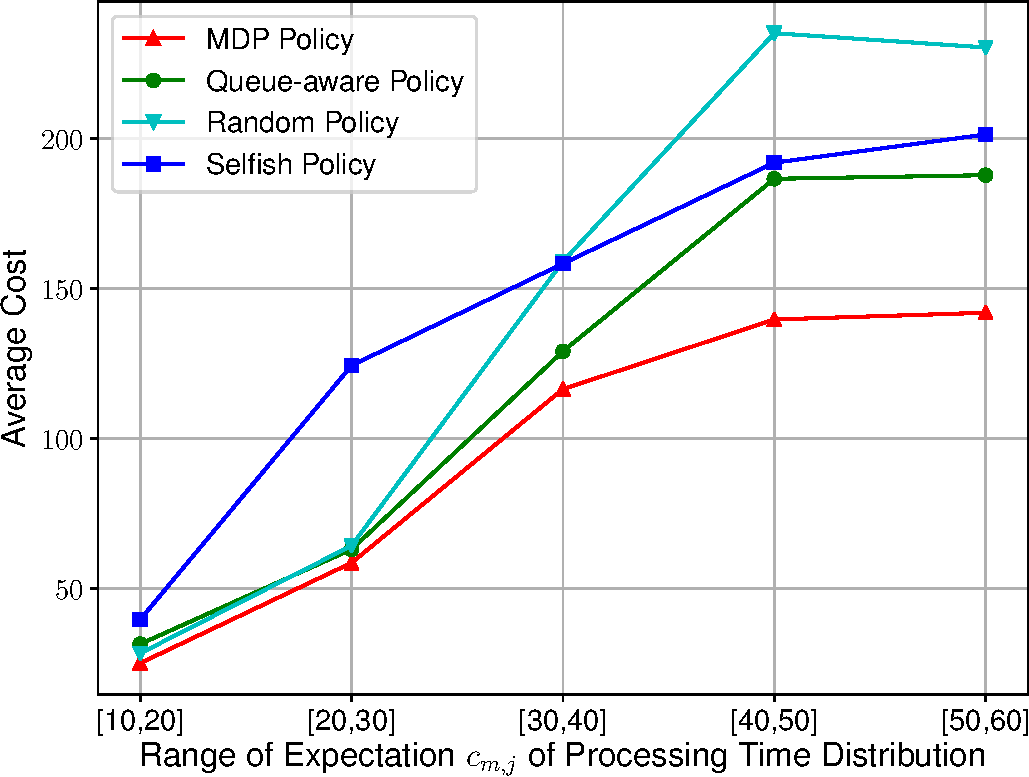
\includegraphics[width=0.45\textwidth]{Study-ProcDist.pdf}      %
    \caption{Illustration of impact of processing time distribution on algorithms.}
    \label{fig:ss_dist}                                             %
\end{figure}                                                        %
%-------------------------------------------------------------------%

% %-------------------------------------------------------------------%
% \begin{figure}[hbt]                                                 %
%     \centering                                                      %
%     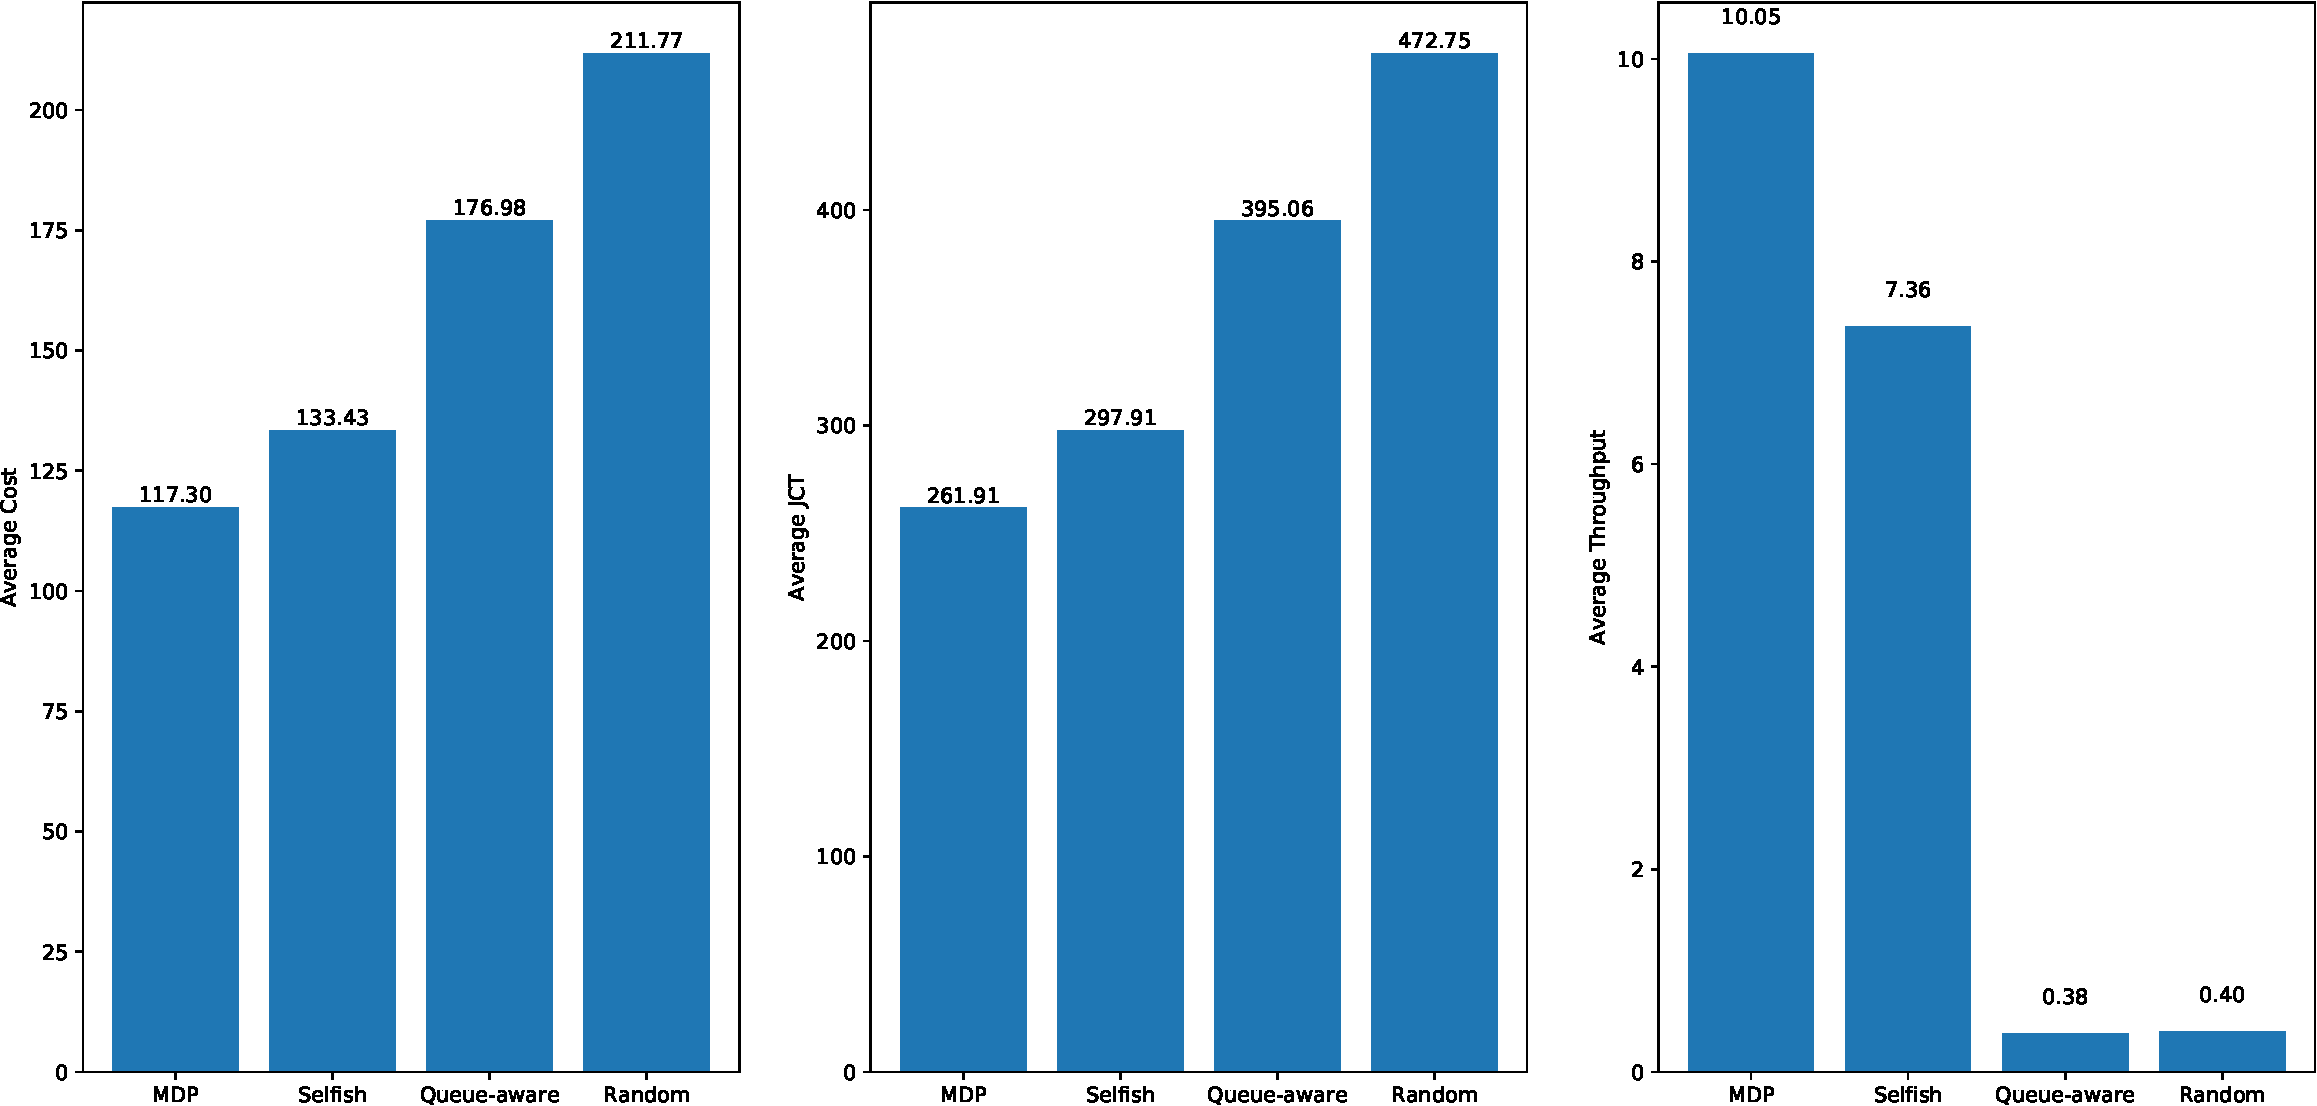
\includegraphics[width=0.45\textwidth]{bar_graph.pdf}           %
%     \caption{Illustration of impact of penalty factors on algorithms.}
%     \label{fig:ss_penalty}                                          %
% \end{figure}                                                        %
% %-------------------------------------------------------------------%

%NOTE: sensitivity study
\textbf{Signaling Latency.}
The simulation results of various support of \brlatency~$\mathcal{D}_{k}$ ($\forall k\in\apSet$) are illustrated in Fig.\ref{fig:ss_delay}.
Specifically, the \brlatency~ of all the APs is set to zero and maximum in in Fig.\ref{fig:ss_delay}(a) and Fig.\ref{fig:ss_delay}(c), respectively.
With the increase of teh \brlatency, \emph{average cost} increase of all the benchmarks and our proposed algorithms.
Overall, the CDF of proposed algorithm is always at the leftmost of the figures under all the situations.
Moreover, the \emph{queue-aware policy} algorithm is sensitive to \brlatency, which performs even  worse than \emph{random policy} algorithm.

\textbf{Number of APs.} %(a.k.a arrival rate)
The simulation results of different sized $K$ of AP set are illustrated in Fig.\ref{fig:ss_scale}.
With the increase of the number of APs, \emph{average cost} increase of all the benchmarks and our proposed algorithms.
Overall, the \emph{average cost} of the proposed algorithm is the smallest under all the situations.
Moreover, the performance of the benchmarks is similar to \emph{random policy} algorithm when the number is smaller than $5$, because the system burden is not heavy.
And the performance of \emph{selfish policy} algorithm is worse than \emph{random policy} algorithm before $K=5$ because it generates a static bipartite graph between the set of APs and edge servers, which actually could not always use all the edge servers.
% {
%     It's shown that on the left of the figure, the SQF algorithm would work better when the system is almost idle; on the right of the figure, SQF and random algorithm could not handle high rejection rate and thus the \emph{average throughput} decreases extremely. 
% }

\textbf{Processing Time Distributions.}
The simulation results of various distributions of processing time are illustrated in Fig.\ref{fig:ss_dist}, where the $c_{m,j}$ of the processing time distribution $\mathbb{G}(1/c_{m,j})$ ($\forall m\in\esSet,j\in\jSpace$) is generated within different ranges.
With the increase of $c_{m,j}$, \emph{average cost} increase of all the benchmarks and our proposed algorithms.
Overall, the \emph{average cost} of the proposed algorithm is the smallest under all the situations.
Moreover, the curves become flat after the range $[40,50]$ because the job rejection penalty domains the cost collected.
Moreover, the performance of \emph{selfish policy} algorithm approaches \emph{queue-aware policy} algorithm when $c_{m,j}$ increases, which shows that the latter could not handle the job rejection situation properly.

% \textbf{Penalty Factors.}
% \fixit{
%     The evaluation of CDF of number of dropped jobs (over the queue limit) is shown in Fig.\ref{fig:ss_penalty}.
%     % tends to job rejection or not
% }

%----------------------------------------------------------------------------------------%
